\documentclass[crop,tikz]{article}
\usepackage{tikz}
\usetikzlibrary{calc,intersections}
\begin{document}

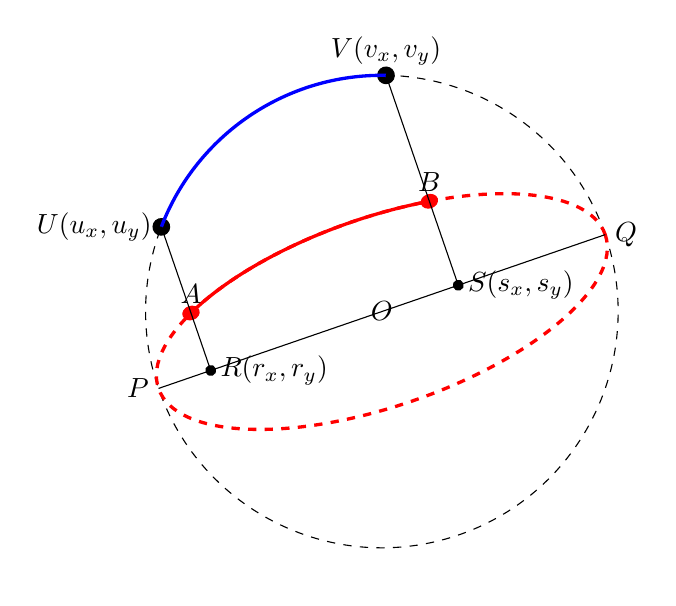
\begin{tikzpicture}[rotate=19]
    \draw[dashed] (0,0) circle (3cm);
    \coordinate (Bc) at (70:3cm);
    \coordinate (Ac) at (140:3cm);
    \coordinate (P) at (-3,0);
    \coordinate (Q) at (3,0);
    \draw[fill] (Ac) circle (3pt);
    \draw[fill] (Bc) circle (3pt);
    \node at (Ac) [above,left] {$U(u_x,u_y)$};
    \node at (Bc) [above] {$V (v_x,v_y)$};
    \node at (P) [left] {$P$};
    \node at (Q) [right] {$Q$};
    \node at (0,0) {$O$};
    \draw[blue,very thick] (Bc) arc (70:140:3cm);
    \begin{scope}[yscale=0.4]
        \draw[very thick,red,dashed] (0,0) circle (3cm);
        \coordinate (Bm) at (70:3cm);
        \coordinate (Am) at (140:3cm);
        \draw[fill,red] (Am) ellipse (3pt and 6pt);
        \draw[fill,red] (Bm) ellipse (3pt and 6pt);
        \draw[red,very thick] (Bm) arc (70:140:3cm);
        \node at (Am) [above] {$A$};
        \node at (Bm) [above] {$B$};
    \end{scope}
    \draw[name path=lineA] (Am) -- (Ac);
    \draw[name path=lineB] (Bm) -- (Bc);
    \draw[name path=majorAxis] (P) -- (Q);
    \coordinate (Ax) at (intersection of Ac--Am and P--Q);
    \coordinate (Bx) at (intersection of Bc--Bm and P--Q);
    \fill (Ax) circle (2pt);
    \fill (Bx) circle (2pt);
    % \fill [blue, name ] circle (2pt);
    \draw (Am) -- (Ax);
    \draw (Bm) -- (Bx);

    \node at (Ax) [below,right] {$R (r_x,r_y)$};
    \node at (Bx) [below,right] {$S (s_x,s_y)$};
\end{tikzpicture}

The red arc $AB$ is a $y$-scaled copy of the blue arc $UV$.

Given the two mouse click positions $A$ and $B$,
the steps to draw line segment (arc) $AB$:
\begin{enumerate}
    \item Compute the cross product $\mathbf N = [N_x, N_y, N_z]$ of the normal vector at $A$ and $B$ to determine the normal vector of the red circle.
    \item Since the ellipse major is on the $XY$ plane and is $\perp$ to $\mathbf N$, we can fix the major axis direction $\vec \mathbf {PQ} = [-N_y, N_x, 0]$
    \item Determine the angle $\alpha$ between $PQ$ and the $X$-axis
    \item Rotate $A$ and $B$ by $-\alpha$, this will let us determine the $(x,y)$-coordinates of the ``unrotated'' copy of $A$ and $B$ and \textbf{after} rotation by $-\alpha$ the following must be true: $a_x = r_x = u_x$  and $b_x = s_x = v_x$ (because $PQ$ now aligns with the $X$-axis)

    \item Since both $U$ and $V$ are on the unit circle, we can calculate the following quantities $u_y = \sqrt{(1 - u_x^2)}$ and $v_y = \sqrt{(1 - v_x^2)}$

\end{enumerate}
\end{document}